\subsubsection{Spenning}
\paragraph{Potensiale} \mbox{} \\
Negativt ladde partikler har en tiltrekkende kraft
og positive partikler har en frastøtende kraft.
Hvis du plasserer en negativ og en positiv partikkel ved siden av
hverandre vil de bli tiltrukket av hverandre. På samme måte
vil to like partikler frastøte hverandre.
\\
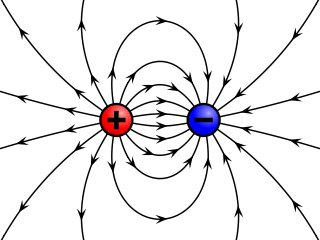
\includegraphics[scale=0.5]{./img/charge}
\\

Et batteri har en negativ og en positiv pol.
Det vil være potensiale for en elektromagnetisk kraft
som trekker de ladde partiklene mot hverandre.
Dette potensialet er hva som kalles spenning.
\\
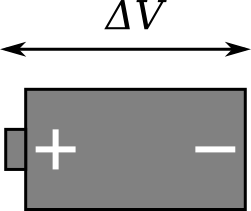
\includegraphics[scale=0.5]{./img/battery}

\paragraph{Enhet} \mbox{} \\
SI enheten for spenning er volt (V) \hfill $\SI{1}{\volt} = J/C$\\
Hvor J står energienheten Joule og C er Coulomb.
